%! Compiler = latexmk -f -r .latexmkrc

\documentclass[
    DIV=13,
    listof=totoc,
    bibliography=totoc,
]{scrreport}

\usepackage{amsmath}
\usepackage{mathtools}
\usepackage{amssymb}

\usepackage[math-style=ISO]{unicode-math}
\usepackage{fontspec}
\setmainfont{TeX Gyre Termes}
\setsansfont{TeX Gyre Heros}
\setmonofont{TeX Gyre Cursor}
\renewcommand{\familydefault}{\sfdefault}
\setmathfont{TeX Gyre Termes Math}

\usepackage{siunitx}

\usepackage{graphicx}
\usepackage{subcaption}

\usepackage{tabularray}
\UseTblrLibrary{booktabs}
\UseTblrLibrary{varwidth}

\usepackage{biblatex}

\addbibresource{refs.bib}
\usepackage{symbols}

\usepackage[hidelinks]{hyperref}

\usepackage[record=nameref,abbreviations]{glossaries-extra}
\usepackage{glossaries}
\GlsXtrLoadResources[src=abbreviations]

\usepackage{textcomp}

\begin{document}
    \title{Microscopic Simulation of Solid State Sintering Regarding Irregularly Shaped Powder Particles}
    \author{Max Weiner}
    \date{\today}

    \maketitle

    \tableofcontents

    \input{tex/preface}

    \printunsrtglossary[type=\glsxtrabbrvtype]

    \chapter{Introduction}\label{ch:introduction}

\section{The RefraBund Project}\label{sec:project-group}
\section{State of the Art}\label{sec:state-of-the-art}

\chapter{Basic Theory of Sintering}\label{ch:basic-theory}

This chapter provides a brief overview of the basic theory of sintering, namely the mechanisms found in sintering processes, the mathematical treatment of those and the modelling of simple particle systems' evolution during sintering.

\input{tex/basic_theory/mechanisms}
\input{tex/basic_theory/diffusion}
\input{tex/basic_theory/thermodynamics}
\input{tex/basic_theory/simple_solutions}

\subsection{Sintering Models with Sharp Interfaces}\label{subsec:sharp-interfaces}
\section{Sintering Models with Diffuse Interfaces}\label{sec:diffuse-interfaces}

\section{Monte-Carlo-Methods (MCM)}\label{sec:monte-carlo}

The term \gls{MCM} refers to a large variety of different methods with the common property to use random numbers as key feature of the algorithm.
\textcite{Lemieux2009} gives a detailed overview about \glspl{MCM} and sampling methods used for them.
Commonly, a distinction is made between Monte-Carlo sampling and Monte-Carlo simulation.
The former uses random numbers following a certain distribution as input to a function to explore the values of the function in the regarded argument space.
The latter uses sampling from distributions to model actual random processes.
According to \textcite{Lemieux2009} these are in fact just two different ways of viewing the problem, the formulation can be converted into each other.
Both will be discuseed in \autoref{subsubsec:monte-carlo-classic}.
A method of this type will be applied for powder modelling in \autoref{ch:powder}.
Another class of methods is often referred to as kinetic \gls{MCM}.
This term refers to modelling the evolution of a system in time by altering the system state in each time step based on random numbers and the probabilities of state change.
This method was used for modelling of sintering and microstructure evolution before (e.g. \cite{Braginsky2005, Luque2010, Tikare2003, Wang2018}), were the probability of state change usually correlates to the local chemical potential.
These methods will be briefly discussed in \autoref{subsubsec:monte-carlo-kinetic-sintering}.

\subsubsection{Classic Monte Carlo Methods}\label{subsubsec:monte-carlo-classic}

The basic idea behind classic \glspl{MCM} is to use randomly sampled values as input to a function and analysing the distribution of result values afterwards using the methods of descriptive statistics.
The
A classic application is the integration of multidimensional functions.
Especially for higher dimensional functions, \glspl{MCM} are much more effective than deterministic, raster-based integration methods like the Newton-Cotes or Gaussian formulae \cite{Lemieux2009}.
\glspl{MCM} need fewer function evaluations to obtain a certain precision than the deterministic raster methods.
The principle is to calculate the average of the function in the regarded interval by estimating the expectation value of the result observations.

Let us consider a function $f$ which is deterministic, but is feeded with a stochastic variable $X$ and maps this to another stochastic variable $Y$ as shown in \autoref{eq:monte-carlo-function}.

\begin{equation}
	Y = f(X)
	\label{eq:monte-carlo-function}
\end{equation}

The variable $X$ is distributed according to a a-priori known distribution with the \gls{PDF} $d_X$ and the \gls{CDF} $D_X$.
To apply a \gls{MCM} one needs to generate a sample $x_i$ of size $N$ which follows this distribution.
The most straightforward way to accomplish this is inversion.
Given a uniformly distributed variable $U$ with samples $u_i$ one may obtain samples of $X$ by applying the inverse of the \gls{CDF} $D_X^{-1}$ as in \autoref{eq:monte-carlo-inversion}.
This method is the simplest and computationally cheapest way of generating such a sample if the inverse \gls{CDF} is available and cheap to compute.
For some distributions, there is no explicit formulation of the \gls{CDF}, most notable for the widely used normal distribution.

\begin{equation}
	x_i = D_X^{-1}(u_i)
	\label{eq:monte-carlo-inversion}
\end{equation}

If inversion is not applicable, there are other methods such as acceptance-rejection and composition.
These are out of the scope of this brief introduction, see \textcite{Lemieux2009} for further information.

To obtain a sample $u_i$ of the uniform variable $U$ one needs a sufficiently good source of random numbers.
One may use lists of real random numbers or hardware random number generators, but usually \gls{PRNG} algorithms are applied.
These are in fact not random, rather deterministic, but the number sequences generated resemble real random sequences well enough.
The main advantage of these algorithms over true random number generators is their repeatability, which means, that the same sequence can be generated multiple times if the same start conditions (seeds) are used.
This enable reproducible calculation results, which is especially useful for debugging und assessment.
Good \gls{PRNG} are characterized by good uniformity of the distribution and high cycle periods.
The actual quality assessment of such generators is a complicated task and out of the scope here.
\textcite{Lemieux2009} gives a brief introduction to this topic and references a large number of more detailed publications.
For this work the Mersenne Twister \cite{Matsumoto1998} was chosen as recommended there.

Evaluation of the function $f$ multiple times with the previously obtained samples $x_i$ as input produces the observations $y_i$ of the variable $Y$. 
These observations are then investigated using classical descriptive statistics.
Special values of interest are often the expectation $\Expectation(Y)$ and the standard deviation or variance $\StandardDeviation(Y)$ resp. $\StandardDeviation(Y)^2$.
Those can be estimated from the sample by \autoref{eq:estimator-expectation} and \autoref{eq:estimator-variance}. 
Note the $N-1$ in \autoref{eq:estimator-variance} for the sample standard deviation, because the naive approach with just $N$ would introduce a bias into the estimation caused by the linking to the estimated expectation $\Estimated\Expectation(Y)$. 
There are several other possibilities to construct estimators for those properties, which may be more efficient (converge to required precision with fewer computational effort) depending on the characteristics of the problem.
Such estimators are known under the term variance reduction techniques, see again \textcite{Lemieux2009} for a overview on these.

\begin{equation}
  \Estimated\Expectation(Y) = \frac{1}{N} \sum_i^N y_i
  \label{eq:estimator-expectation}
\end{equation}

\begin{equation}
  \Estimated\StandardDeviation^2(Y) = \frac{1}{N-1} \sum_i^N \left( y_i - \Estimated\Expectation(Y) \right)^2
  \label{eq:estimator-variance}
\end{equation}

\subsubsection{Sintering Simulation by Kinetic Monte Carlo Methods}\label{subsubsec:monte-carlo-kinetic-sintering}

The basic idea behind most kinetic \glspl{MCM} (f.e. \cite{Braginsky2005, Luque2010, Tikare2003, Wang2018}) is to discretize the model space into finite volumes (voxels) with a defined discrete state, which may change with a defined probability. 
This type of system discretization is also referred to as cellular automaton.
In each step, a voxel is chosen randomly and the probability of changing its state is calculated. 
Then, the state is changed conditionally by comparing the probability to the value of a random number. 
The term "kinetic" refers hereby to the correlation of the number of steps performed to the process time. 
This correlation is usually not directly obtainable, but has to be determined by comparison to experimental results, if desired.

The way to determine the probability of state changes varies in the publisched models. 
\citeauthor{Braginsky2005}\cite{Braginsky2005, Tikare2003} evaluate the energy change $\Diff E$ of the system for the case the state change has actually happened.
The energy change is then correlated to the probabilty by \autoref{eq:kinetic-monte-carlo-energy-probability}, where a negative ernergy change (reduction of system energy) is always accepted, however positive ones tend to zero probability by an exponential law.  

\begin{equation}
  \Probability = \begin{cases}
    \exp \left( -\frac{\Diff E}{\BoltzmannConstant \Temperature} \right) & \Diff E > 0 \\
    1 & \Diff E \le 0
  \end{cases}
  \label{eq:kinetic-monte-carlo-energy-probability}
\end{equation}

Another way correlates the probability to the local surface geometry, which resembles classic sintering theory. 
\textcite{Luque2010} (although for liquid phase sintering) evaluates the number of neighboring voxels with the same or different state and correlate the probability with that count. 
High count of non-solid (in this case liquid, but void also imaginable) voxels beneath a solid mean a high convex curvature at this point. 
In contrast, a high count of solids beneath a a non-solid one mean a high concave curvature.
In \textcite{Luque2005}, they evaluate a number of different approaches for the correlation between these counts and the probability. 
They remark, that although lots of different approaches could be chosen, only few are feasible due to the danger of generating numerical artifacts in the system state.
A similar approach was taken by \textcite{Wang2018}.

This type of models is especially usefull for liquid phase sintering, since there are no voids, so state change from liquid to solid or vice versa does not violate the mass conservation law. 
In solid state sintering one has to make sure, that for every solid voxel appearing there is one removed. 
Especially to model densification void voxels have to be transported to the outer surface. 
\textcite{Braginsky2005} remove a solid voxel at the outer surface for every vacancy anhilated at a grain boundary. 
This approach, although conserving the mass, appears like teleportation of mass from the surface to the inner and lacks therefore in physical justification.

The main difficulty of these models is the mapping of the internal time of the algorithm, often referred to as Monte Carlo steps (MCS), to the actual time of the real process. 
The models usually do not involve any kinetic parameters like diffusion coefficients or mobilities, as they are not required for the solution of the model. 
However, this complicates the transfer of the simulation results to the experiment or comparision to other simulation approaches.
Usually, a linear correlation between MCS and real time is assumed and the proportionality factor is fitted by experiments or other simpler models.

\subsection{The Thermodynamic Extremal Priciple (TEP)}\label{subsec:extremal-priciple}

\subsubsection{Classic Formulation}\label{subsubsec:extremal-priciple-classic}

\subsubsection{Generalized Formulation}\label{subsubsec:extremal-priciple-generalized}

\subsection{Miscellaneous}\label{subsec:miscellaneous}


    \chapter{Aim and Scope}\label{ch:aim-and-scope}

The work aims on the following goals:
\begin{enumerate}
    \item Develop a model for the microscopic sintering behavior of mutliple particles.
    \item Implement a reusable software framework for its application.
    \item Investigate its numerical behavior and define feasible numerical control parameters.
    \item Investigate its physical predictions, explain and compare them with literature results.
    \item Develop a method for statistical representation of powders using the sintering model to allow design of powder mixtures.
\end{enumerate}

\section{Requirements to the Model}\label{sec:requirements}

The work resides under the circumstances of the RefraBund project, where a composite refractory material consisting of alumina and metallic niobium or tantalum is developed.
From these circumstances the following requirements and assumptions are derived:
\begin{description}
    \item[Diffusion Mechanisms] The model shall regard surface and grain boundary diffusion as the two main mechanisms of solid state sintering for metallic and ceramic materials.
        Volume diffusion is neglected, as it is commonly slow compared to surface or grain boundary.
        The effect of grain boundary diffusion was compared by \textcite{Fisher1951} with \emph{the heat flux in a foil of copper embeded in cork}.
        Other mechanisms like evaporation-condensation or vicose flow do not have to be expected.
    \item[Asymmetric Geometry Contacts] The model shall support particles of arbitrary shape and different size.
        The first shall allow the investigation of the influence of non-ideal particle geometries.
        Size differences are to be limited to one or two orders of magnitude to avoid major numerical complications in terms of discretization widths.
        These requirements drop the use of any symmetry assumptions which are often applied in literature models.
    \item[Asymmetric Material Contacts] The investigated material consists of alumina powder as well as metallic niobium resp.~tantalum powder.
        The model must therefore be able to respect different material properties on particles in contact to each other with their implication of grain boundary shape and kinetic behavior.
        However, the materials are assumed to be insoluable in each other to avoid regard on concentration gradients within the particles.
        Mass transfer between particles is therefore also disregarded.
    \item[Multi-Particle-Contacts] As the often applied two-particle approach neglects important influences, especially pore closing and mutual hindering of particles in their evolution.
        The latter is referred to the mutual influence of multiple contacts, which differ in their geometry and/or material characteristic and so can not be regarded as isolated anymore.
    \item[Powder Mixture] The production process involves mixing of different powder fractions to obtain optimal properties in processing and application.
        The development of a sintered material and its processing heavily resides on determining the ideal mixture to be used for the regarded application.
        The model should be able to regard different mixtures to try them out in simulation instead of laboratory.
\end{description}
The model shall be restricted to 2D-space as a proof of concept, but may be extended to 3D-space as well.
The latter is out of scope of this work.

\section{Rational on Approach and Methods}\label{sec:rational-on-approach-and-methods}

The model development of the current work shall reside on a direct and sharp interface description by using the \glsfirst{FDM}.
The main reason for this is the avoidance of a unphysically wide diffuse interface, as would come with the application of the major competitor: the \glsfirst{PFM}.
The work shall explore the influence of concrete physical material parameters, which are included in sharp interface approaches directly, rather then requiring an additional mapping to fit into the numeric scheme.
The latter would introduce additional errors that could be avoided.
Volume diffusion is not needed, so no discretization of the bulk material.
Therefore, choosing a \gls{FEM} discretization instead of \gls{FDM} for the surface line only seems to be to much effort.
Application of the \glsfirst{LSM} can be discarded due to the lack of support for multiple phases and grains.

For getting a clean and concise mathematical formulation, as would come with the \gls{PFM}, on top of this numerical system representation the \glsfirst{TEP} shall be applied to construct the governing equations of temporal system evolution.
This concept has already been successfully applied to similar problems.
In the current case the complexity of the system will significantly rise in comparison to earlier applications, since the number of state variables will drastically increase.
The concept has the main benefit of easy implicit incorporation of additional constraints arising from contact geometry requirements and boundary conditions.

To model the powder properties regarding size and shape of the particles, a statistical approach based on the \glsfirst{MCM} shall be taken.
Random generation of particles subject to a statistical representation of the powder characteristics shall link the microscopic model, restricted to small counts of particles, to the macroscopic world.
Independent simulation of multiple draws enable furthermore parallel computing with low effort, since now attention has to be given to concurrent memory access.
The problem of calculating a large \glsfirst{RVE} with many particles shall be reduced to calculating multiple \glsplural{RVE} with fewer particles and characterizing their behavior by methods of descriptive statistics.

    \chapter{Powder Analysis and Representation}\label{ch:powder}

\section{Classic Methods of Powder Characterization}\label{sec:classic-methods}
\section{Particle Description by Parametrized Shape Functions}\label{sec:shape_functions}
\section{Characterization of Powder Properties}\label{sec:powder-characterization}


    \chapter{Model Development}\label{ch:model-development}

\section{A Discrete Model of Powder Particles}\label{sec:particle-model}

\begin{itemize}
    \item Particles, Coordinate System
    \item Node Types
    \item Multi-Scale Considerations, Matrix
\end{itemize}

Continuous description of the particle surface geometry is only possible for nearly ideal geometries.
For complicated geometries a discretized approach is feasible.
For the current work, the concept of a node shall be introduced.
A node is here considered as a discrete point of the particle surface connected with its neighbors by straight lines.
The spline of those lines is defining the surface of the particle.

The location of each node in space is defined by a tuple of polar coordinates $(\Angle, \Radius)$, where $\Angle$ is the angle coordinate and $\Radius$ the radius resp.~distance from origin.
The origin of the polar coordinates is distinct for each particle and is considered as the center of the particle, although it is generally not identical with the barycenter of the particle.
But the center of the particle is used as an anchor for defining a particles postions in space.
With this concept the particle can be moved in space without translating the surface node coordinates and the description of node evolution is simplified, since only the local geometry must be regarded.
Particle movement occurs due to diffusional fluxes in the grain boundaries, which is macroscopically observed as shrinkage.

The location of a particle is defined by the cartesian coordinates of its center $\X$ and $\Y$, as well as a rotation angle $\RotationAngle$ with the center as pole.
The rotation angle also defines the origin axis of the particles local coordinate system.

The contact topology of multiple particle can be described as a graph, where the vertices correspond to particles and the edges correspond to contact relations between the particles.
The undirected graph structure of a particle contact is shown in \autoref{fig:model_development/particle_graph}.
The indices of the vertices are at this point arbitrary, but are reused in the same way in the following.

For simulation purposes, the introduction of a hierarchy in the particle contacts is feasible to introduce a specific order for equation construction.
More specifically the particle contacts shall be described as a~\gls{DAG}.
Such a graph can always be constructed from a given undirected graph by performing a \gls{BFGS} starting at the desired root vertex and dropping all edges pointing back to the parent.
An example of such a structure in shown in \autoref{fig:model_development/particle_graph_dag}.
The particle labeled with index 0 is the \emph{root} of the graph, the only vertex that has no incoming edges.
In general, the root of the particle graph can be chosen arbitrarily, but for efficiency reasons, it should be a particle which leads to a graph as flat as possible.
The root particle has a fixed position in space and therefore acts as origin for all coordinate systems used throughout the calculations.
There may be cases, where the particle graph has rooted tree structure, which simplifies the problem significantly, since then all particles are able to move freely.
Edges like the red one in the figure break the tree structure.
Note, that they do not form cycles in the~\gls{DAG} in the meaning of graph theory, since the edges are directed.
But in terms of the underlying undirected graph they are anyway cycles.
To avoid ambiguities, the term ring contact shall be used here instead.
Ring contacts introduce additional constraints to the particle movement, since each particle in the ring influences the movement of the others.
The edges closing a ring are named correspondingly as \glspl{RCE}.

\begin{figure}
    \centering
    \includegraphics{img/model_development/particle_graph}
    \caption{Undirected Particle Graph Representing Contact Conditions}
    \label{fig:model_development/particle_graph}
\end{figure}

\begin{figure}
    \centering
    \includegraphics{img/model_development/particle_graph_dag}
    \caption{Directed Acyclic Graph Structure of Particle COntacts Rooted at Vertex 0}
    \label{fig:model_development/particle_graph_dag}
\end{figure}

\Glspl{RCE} are discovered during a~\gls{BFGS} when a vertex is encountered that was already marked as visited.
To be able to construct geometric constraints on particle movement, a ring path must be defined.
A ring path is a path following the cycle in the undirected graph, the currently regarded ring corresponds to.
It is generally not unique, but this is also not necessary.
To find a ring path, a~\gls{DFGS} is performed on the undirected particle graph with the ring closing edge removed.
The removed edge is afterwards appended to the path to close the ring.
The procedure is illustrated in \autoref{fig:model_development/particle_graph_ring_search}.

\begin{figure}
    \centering
   % \includegraphics{img/model_development/particle_graph_ring_search}
    \caption{Ring Path Search Using a Depth-First Graph Search}
    \label{fig:model_development/particle_graph_ring_search}
\end{figure}

In regard of sintering processes, the contact properties of multiple particles are investigated.
The common interface of two particles in contact is commonly called a sinter neck.
It consists of a grain boundary bounded by triple points of the grain boundary and the two adjacent free surfaces.
Until here, three types of nodes can be identified:
\begin{description}
    \item[Surface Nodes] forming the free surface of a particle in contact to atmosphere or vacuum.
    \item[Grain Boundary Nodes] forming the grain boundary in a particle contact.
    \item[Neck Nodes] representing the triple point between grain boundary and two surfaces.
\end{description}
Details on the conditions at those nodes are given in the following sections.

\section{Considerations on Free Surfaces}\label{sec:free-surfaces}

\begin{figure}
    \centering
    \includegraphics{img/model_development/neck-normal}
    \caption{}
    \label{fig:model_development/time_step_neck_normal}
\end{figure}
\section{Considerations on Grain Boundaries}\label{sec:grain-boundaries}

In contrast to free surfaces, where the geometric evolution of a node is not constrained by the surrounding space, in grain boundaries the node shifting acts counter the solid material of the other particle.
This introduces additional constraints, since the grain boundary must not form holes and must not overlap.
The geometric constraints are dependent on the local evolution of the grain boundary nodes, as well as the relative position change of the particles.

Starting from a compact grain boundary, meaning that there are no holes and/or overlap present within it, the condition of maintaining the compactness of the grain boundary can be formulated as follows, if the postions of the particles are fixed.

\begin{align}
	\Step\Shift_{\Normal}\Regarding\Parent = -\Step\Shift_{\Normal}\Regarding\Child \\
	\Step\Shift_{\Tangential}\Regarding\Parent = -\Step\Shift_{\Tangential}\Regarding\Child
	\label{eq:maintain-compact-particles-fixed}
\end{align}

But in reality the positions of particles to each other change, which can be observed macroscopically as shrinkage.
However, the relation between node shifting and particle movement cannot be easily formulated, since the particle movement is effected by the ensemble of all nodes involved in the contact.
But, we can formulate the influence of shifting one single node in normal or tangential direction on the particles' relative postion, if we assume that the other nodes do to hinder movement.
Each contact node has two sets of coordinates, one in the terms of the one particle, one in terms of the other.
However, they represent both the same point in space.

\autoref{fig:model_development/particle_shift_normal} and \autoref{fig:model_development/particle_shift_tangential} show the geometric conditions of such a shift.
The parent particle (index ${\Parent}$) changes its shape by shifting a single regarded node (green), as the child particle (index ${\Child}$) also (red).
The particles are assumed to be solely connected in the regarded node, the influence of adjacent nodes is disregarded.
If the new positions of the nodes are put in alignment again, one observes a relative movement of the particles' centers equal to the difference of both node shifting vectors.
This particle center shift leads to a change in contact distance $\Step\Radius_{{\Contact}} = \Radius'_{\Contact} - \Radius_{\Contact}$ and direction $\Step\Angle_{\Contact}\Regarding\Parent$.
The child particle experiences the same direction step as the parent $\Step\Angle_{\Contact}\Regarding\Parent = \Step\Angle_{\Contact}\Regarding\Child$.
The shifting of one node alone does not affect a rotation of the child particle, but the ensemble of node shifts above and below the contact line.
Therefore, the rotation step $\Step\RotationAngle_{\Child}$ is introduced as another auxiliary variable, whose effect on particle center shift is as in \autoref{fig:model_development/particle_shift_rotation}.

The total movement of the right particle due to node shifting can be formulated as a total differential:
\begin{subequations}
	\begin{align}
		\Step\Radius_{\Contact}           & =
		\frac{\partial \Radius_{\Contact}}{\partial \Shift_{\Normal}\Regarding\Parent} \Step\Shift_{\Normal}\Regarding\Parent
		+ \frac{\partial \Radius_{\Contact}}{\partial \Shift_{\Normal}\Regarding\Child} \Step\Shift_{\Normal}\Regarding\Child
		+ \frac{\partial \Radius_{\Contact}}{\partial \Shift_{\Tangential}\Regarding\Parent} \Step\Shift_{\Tangential}\Regarding\Parent
		+ \frac{\partial \Radius_{\Contact}}{\partial \Shift_{\Tangential}\Regarding\Child} \Step\Shift_{\Tangential}\Regarding\Child
		+ \frac{\partial \Radius_{\Contact}}{\partial \Shift_\RotationAngle} \Step\Shift_\RotationAngle \\
		%
		\Step\Angle_{\Contact}\Regarding\Parent & =
		\frac{\partial \Angle_{\Contact}\Regarding\Parent}{\partial \Shift_{\Normal}\Regarding\Parent} \Step\Shift_{\Normal}\Regarding\Parent
		+ \frac{\partial \Angle_{\Contact}\Regarding\Parent}{\partial \Shift_{\Normal}\Regarding\Child} \Step\Shift_{\Normal}\Regarding\Child
		+ \frac{\partial \Angle_{\Contact}\Regarding\Parent}{\partial \Shift_{\Tangential}\Regarding\Parent} \Step\Shift_{\Tangential}\Regarding\Parent
		+ \frac{\partial \Angle_{\Contact}\Regarding\Parent}{\partial \Shift_{\Tangential}\Regarding\Child} \Step\Shift_{\Tangential}\Regarding\Child
		+ \frac{\partial \Angle_{\Contact}\Regarding\Parent}{\partial \Shift_\RotationAngle} \Step\Shift_\RotationAngle
	\end{align} \label{eq:particle-steps}
\end{subequations}
The partial derivatives therein are obtained from the geometric relations in the above figures.


Of course, for each node the resulting movement of the particle will be different due to geometric relations and diffusive fluxes.
The geometric relations are fixed for a regarded state, but the diffusive fluxes can be used to fulfill \autoref{eq:particle-steps} simultaneously for all nodes involved in a contact.
So there is a set of equations available to describe particle contact conditions as constraints for the TEP-approach.

\begin{equation}
	\Radius'_{{\Contact}} = \sqrt{\Radius_{{\Contact}}^2 + \Step\Shift^2 - 2 \Radius_{{\Contact}} \Step\Shift \cos \eta}
	\label{eq:contact-rcprime-normal}
\end{equation}

\begin{equation}
	\Step\Angle_{{\Contact}}\Regarding\Parent = \arcsin \left[ \frac{\sin \eta}{\Radius'_{\Contact}} \Step\Shift \right]
	\label{eq:contact-dphic-normal}
\end{equation}

\begin{equation}
	\frac{\partial \Radius_{\Contact}}{\partial \Shift}
	= \lim_{\Step\Shift \rightarrow 0} \frac{\Radius'_{\Contact} - \Radius_{\Contact}}{\Step\Shift}
	= - \cos \eta
	\label{eq:contact-partial-rc-normal}
\end{equation}

\begin{equation}
	\frac{\partial \Angle_{\Contact}\Regarding\Parent}{\partial \Shift}
	= \lim_{\Step\Shift \rightarrow 0} \frac{\Step\Angle_{\Contact}\Regarding\Parent}{\Step\Shift}
	= \frac{\sin \eta}{\Radius_{\Contact}}
	\label{eq:contact-partial-dphi-normal}
\end{equation}

These constraints can also be seen as a different formulation of the force balance on the grain boundary.
An additional contraint arrises from the torque balance, which dertermines the rotation of the child particle around its center. 
Each mode of node shifting induces a torque on the child particle, which depends on the size of the shift, the local radius of the particle and the orientation of surface and shift.
The particular torques as given in \autoref{eq:particular-torque} must balance to zero for each contact (\autoref{eq:torque-balance}).
$\Projected\Radius\Regarding\Child$ is the projected lever arm of the particular shift relative to the child particle's center,
the actual prescription to calculate depends on the mode of shift an will be given below.

\begin{equation}
  \Torque = \Step\Shift \cdot \Projected\Radius\Regarding\Child
  \label{eq:particular-torque}
\end{equation}

\begin{equation}
	\sum^{\Nodes_{\Contact}} \Radius\Regarding\Child
	\left[
		\Step\Shift_{\Normal}\Regarding\Parent \cos \left( \SurfaceRadiusAngle_{\Upper}\Regarding\Child + \frac\pi2 - \SurfaceVectorAngle_{{\Normal}{\Lower}}\Regarding\Parent\right)
		+ \Step\Shift_{\Normal}\Regarding\Child \cos \left( \SurfaceRadiusAngle_{\Upper}\Regarding\Child + \SurfaceVectorAngle_{{\Normal}{\Upper}}\Regarding\Child - \frac\pi2 \right)
		+ \Step\Shift_{\Tangential}\Regarding\Parent \cos \left( \SurfaceRadiusAngle_{\Lower}\Regarding\Child - \frac\pi2 - \SurfaceVectorAngle_{{\Tangential}{\Upper}}\Regarding\Parent\right)
		+ \Step\Shift_{\Tangential}\Regarding\Child \cos \left( \frac\pi2 - \SurfaceRadiusAngle_{\Upper}\Regarding\Child - \SurfaceVectorAngle_{{\Tangential}{\Upper}}\Regarding\Child\right)
		\right]
	= 0
	\label{eq:torque-balance}
\end{equation}

In the following, the geometric relations will be derived for each of the node shift modes.

\subsection{Normal Shifting}

\begin{figure}
	\begin{subfigure}{\linewidth}
		\centering
		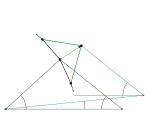
\includegraphics{img/model_development/particle_shift_normal}
		\caption{Parent's Node}
		\label{fig:model_development/particle_shift_normal/parent}
	\end{subfigure}
	\begin{subfigure}{\linewidth}
		\centering
		\includegraphics{img/model_development/particle_shift_normal_child}
		\caption{Child's Node}
		\label{fig:model_development/particle_shift_normal/child}
	\end{subfigure}
	\caption{Effect of Normal Node Shifting on Particle Postion}
	\label{fig:model_development/particle_shift_normal}
\end{figure}

\begin{equation}
	\eta_{\Normal}\Regarding\Parent = \PI - \left( \Angle\Regarding\Parent - \Angle_{\Contact}\Regarding\Parent \right) + \left( \PI - \SurfaceVectorAngle_{\Normal}\Regarding\Parent - \SurfaceRadiusAngle_{\Lower}\Regarding\Parent \right)
	\label{eq:contact-eta-normal-parent}
\end{equation}

\begin{equation}
	\eta_{\Normal}\Regarding\Child = \PI + \left( \Angle_{\Contact}\Regarding\Child - \Angle\Regarding\Child \right) - \left( \PI - \SurfaceVectorAngle_{\Normal}\Regarding\Child - \SurfaceRadiusAngle_{\Upper}\Regarding\Child \right)
	\label{eq:contact-eta-normal-child}
\end{equation}

\subsection{Tangential Shifting}

\begin{figure}
	\begin{subfigure}{\linewidth}
		\centering
		\includegraphics{img/model_development/particle_shift_tangential}
		\caption{Parent's Node}
		\label{fig:model_development/particle_shift_tangential/parent}
	\end{subfigure}
	\begin{subfigure}{\linewidth}
		\centering
		\includegraphics{img/model_development/particle_shift_tangential_child}
		\caption{Child's Node}
		\label{fig:model_development/particle_shift_tangential/child}
	\end{subfigure}
	\caption{Effect of tangential Node Shifting on Particle Postion}
	\label{fig:model_development/particle_shift_tangential}
\end{figure}

\begin{equation}
	\eta_{\Tangential} = \PI - \left( \Angle\Regarding\Parent - \Angle_{\Contact}\Regarding\Parent \right) - \left( \PI - \SurfaceVectorAngle_{\Tangential}\Regarding\Parent - \SurfaceRadiusAngle_{\Upper}\Regarding\Parent \right)
	\label{eq:contact-eta-tangential-parent}
\end{equation}

\begin{equation}
	\eta_{\Tangential} = \PI + \left( \Angle_{\Contact}\Regarding\Child - \Angle\Regarding\Child \right) - \left( \PI - \SurfaceVectorAngle_{\Tangential}\Regarding\Child - \SurfaceRadiusAngle_{\Upper}\Regarding\Child \right)
	\label{eq:contact-eta-tangential-child}
\end{equation}

\subsection{Particle Rotation}

\begin{figure}
	\centering
	\includegraphics{img/model_development/particle_shift_rotation}
	\caption{Effect of Particle Rotation on Particle Postion}
	\label{fig:model_development/particle_shift_rotation}
\end{figure}

\begin{equation}
	\Step\Shift_{\RotationAngle} = 2 \Radius\Regarding\Child \sin \frac{\Step\RotationAngle_{\Child}}{2}
	\label{eq:contact-ds-rotation}
\end{equation}

\begin{equation}
	\eta_\RotationAngle = -\left( \Angle\Regarding\Child - \Angle_{\Contact}\Regarding\Child \right) + \frac{\PI - \Step\RotationAngle_{\Child}}{2}
	\label{eq:contact-eta-rotation}
\end{equation}

% TODO simplified equations




\section{Considerations on Sinter Necks}\label{sec:necks}

\section{Considerations on Grain-Matrix Interfaces}\label{sec:grain_matrix}

\begin{figure}
    \begin{center}
        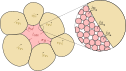
\includegraphics[width=0.95\textwidth]{img/model_development/grain_matrix_overview}
    \end{center}
    \caption{Principle of the Multiscale Approach with Coarse Particle Skeleton and Fine Particle Matrix Continuum}\label{fig:model_development/grain_matrix_overview}
\end{figure}

Since the investigated material is characterized by particle sizes in several orders of magnitude (fine alumina with $\Diameter \approx \qty{20}{\micro\meter}$ and aggregates with $\Diameter \approx \qty{2}{\milli\meter}$), direct simulation of contact between all possible occuring particles is not possible.
A fine discretization on all particles would lead to excessive high count of nodes on the coarse particles.
A coarse discretization on all particles would lead to a degenerated shape of the small ones.
A fine discretization on small ones and a coarse on large ones, however, would lead to large numerical errors in contacts due to heavily different discretization widths on both sides.
Therefore, another approach has to be taken.

In the following, a multiscale approach consisting of a finely powdered continuum matrix and a skeleton of large particles shall be developed
The idea is illustrated in \autoref{fig:model_development/grain_matrix_overview}.
From the view of the large particles, the fine fractions of the powder mixture behave like a continuum, however a porous one, which shows its own sintering behavior.
The behavior of the matrix can be described in different ways.
The simplest approach is to describe it by some simplified sintering model like empirical power laws or circular two-particle models.
The more detailed way is to use the same model as proposed for the large grains for the small ones alone while neglecting the presence of the large.
This approach enables a cascading model hierachy while going down from the largest to the smallest particles while considering the current large fraction as skeleton.

The following relations in sintering behavior between the fractions have to be kept in mind:
\begin{itemize}
    \item The time scale of the matrix' sintering is much faster than that of the skeleton because of the smaller grain size (which contributes by power of four to the sintering time scale).
    \item Grain coarsening (final sintering stage) may occur in the matrix while the skeleton is still in initial or intermediate stage.
    \item The matrix hinders the free movement of the skeleton particles, additonally to the hindering of ring-type contacts within the skeleton. This results in additonal stresses on the skeleton particle surface.
    \item Substance will diffuse from the matrix to the skeleton particles, especially contributing to the growth of the neck, but also equalizing surface structures.
    \item Occupancy of skeleton particle surface by matrix will influence their effective surface diffusion coefficient and surface energy.
\end{itemize}

\subsection{Estimation of Stress on Skeleton Surfaces}

\subsection{Estimation of Effective Skeleton Surface Properties}

\section{Application of the Thermodynamic Extremal Principle}\label{sec:extremal-principle-application}

In the following the generalized extremal principle is applied on the current model of particles and nodes, see \autoref{subsubsec:extremal-priciple-generalized} for details on the approach.
As before, an index of the currently regarded particle or node is neglected where appropriate for brevity.
The indizes $\ldots_{\Upper}$ and $\ldots_{\Lower}$ are used to denote the upper resp.~lower neighbor of a node.
${\Nodes}$ is the set of all nodes present in the system and ${\Particles}$ the set of all particles, respectively.

\subsection{Choice of Variables}\label{subsec:choice-of-variables}

First, the internal state variables $\Vect\InternalStateVariable$, the internal state velocities $\Vect\InternalStateVelocity$ and the fluxes $\Vect\Flux$ must be chosen.
The feasibility of the approach heavily depends on this choice.

The choice of the fluxes is straightforward with the diffusional fluxes.
One has two diffusional fluxes on each node $\Flux_{\Upper}$ and $\Flux_{\Lower}$, however the flux of the upper node to the lower and the flux from the lower to the upper are always equal due to constance of mass.
Additional fluxes are to be found in the fluxes from the particle to the matrix $\Flux_{\Matrix}$, if a matrix is present in the inter-particle spaces.

The internal state variables are the polar coordinates of the nodes $\left[ \Radius, \Angle \right]$ with pole in their particle's center, since they determine the thermodynamic forces and the main aim of the simulation is to follow the time evolution of the particles and nodes.
The coordinates of the particles $\left[ \Radius_{\Particle}, \Angle_{\Particle}, \RotationAngle_{\Particle} \right]$ are not used as internal state variables, since they are unambiguously defined, if the coordinates of all nodes relative to their particle are known and also which nodes are in contact to each other.
Moreover, the particle coordinates are auxiliary variables (included in $\Vect\AuxiliaryVariable$) to ease formulation of the geometric constraints.

For numerical and equation formulation reasons, the internal state velocities $\dot\Radius$ and $\dot\Angle$ are replaced by the velocities of node shift along normal and tangential surface vectors $\dot\Shift_{\Normal}$ and $\dot\Shift_{\Tangential}$.
As they are determined, translation into new coordinates is directly possible using the relations obtained in the previous sections.

The external state variables (such as temperature $\Temperature$ and pressure $\Pressure$) are not considered in the following, since they are assumed constant.

\subsection{Establishing the Equation System}

In the following the necessary equations shall be composed.
This includes the definition of the dissipation $\Dissipation$, the dissipation function $\DissipationFunction$, required constraints and additional constraints.
The resulting components of the Lagrangian gradient and the respective Jacobian matrix are omitted here for brevity, but listed in \autoref{ch:equation-system}.

\minisec{Dissipation $\Dissipation$}

The dissipation at one node is given by the product of node shifts and the respective Gibbs energy derivatives as in \autoref{eq:dissipation-node}.
The Gibbs energy derivatives were determined in \autoref{sec:surface-evolution} for the different node types.
The dissipation of the whole system is the sum of all node dissipations, since all thermodynamic forces occur at nodes.
Shifting of particles alone does not follow a thermodynamic force, but is determined by the ensemble of the involved nodes.

\begin{equation}
    \Dissipation = -\sum^{\Nodes} \left[ \frac{\partial \GibbsEnergy}{\partial \Shift_{\Normal}} \dot\Shift_{\Normal} + \frac{\partial \GibbsEnergy}{\partial \Shift_{\Tangential}} \dot\Shift_{\Tangential} \right]
    \label{eq:dissipation-node}
\end{equation}

\minisec{Dissipation Function $\DissipationFunction$}

The dissipation function as formulation of the dissipation in terms of fluxes involves the square of fluxes,
the surface distance $\SurfaceDistance$,
the diffusion coefficient along the interface $\DiffusionCoefficient$,
the molar volume $\MolarVolume$ of the particle substance,
the thermal vacancy concentration $\VacancyConcentration^{\Standard}$ at the respective temperature,
the universal gas constant $\GasConstant$
and the absolute temperature $\Temperature$.
Regarding only the fluxes to the upper node is sufficient, since the fluxes to the lower are regarded from the lower node on.

\begin{equation}
    \DissipationFunction = \sum^{\Nodes} \frac{\GasConstant\Temperature}{\MolarVolume{\VacancyConcentration}^\Standard} \frac{\SurfaceDistance_{\Upper} {\Flux}_{\Upper}^2}{{\DiffusionCoefficient}_{\Upper}}
    \label{eq:dissipation-function-node}
\end{equation}

The Langrangian multiplicator for the equality constraint of both dissipation formulations will be denoted as $\LagrangeParameter_{\Dissipation}$ in the following.

\minisec{Required Constraints $\Vect\RequiredConstraint$}

The required constraints needed to link internal state velocities and fluxes are given by the constance of volume resp.\ mass at each node.

\begin{equation}
    \frac{\partial\Volume}{\partial{\Shift}_{\Normal}} {\dot\Shift}_{\Normal} + \frac{\partial\Volume}{\partial{\Shift}_{\Tangential}} {\dot\Shift}_{\Tangential} = \dot\Volume = \left( {\Flux}_{\Upper} + {\Flux}_{\Lower} \right)
    \label{eq:required-constraint-flux-shift}
\end{equation}

The Langrangian multiplicator for this constraint will be denoted as $\LagrangeParameter_\Volume$ in the following.

\subsection{Additonal Constraints $\Vect\AddionalConstraint$}\label{subsec:additonal-constraints}

Additional constraints occur at particle contacts.
For each node involved in a contact the conditions according to \autoref{eq:particle-steps} are applied in a formulation in terms of node shift velocities $\dot\Shift$.

\begin{subequations}
    \begin{align}
        \dot\Radius_{\Contact}           & =
        \frac{\partial \Radius_{\Contact}}{\partial \Shift_{\Normal}\Regarding\Parent} \dot\Shift_{\Normal}\Regarding\Parent
        + \frac{\partial \Radius_{\Contact}}{\partial \Shift_{\Normal}\Regarding\Child} \dot\Shift_{\Normal}\Regarding\Child
        + \frac{\partial \Radius_{\Contact}}{\partial \Shift_{\Tangential}\Regarding\Parent} \dot\Shift_{\Tangential}\Regarding\Parent
        + \frac{\partial \Radius_{\Contact}}{\partial \Shift_{\Tangential}\Regarding\Child} \dot\Shift_{\Tangential}\Regarding\Child \\
        %
        \dot\Angle_{\Contact}\Regarding\Parent & =
        \frac{\partial \Angle_{\Contact}\Regarding\Parent}{\partial \Shift_{\Normal}\Regarding\Parent} \dot\Shift_{\Normal}\Regarding\Parent
        + \frac{\partial \Angle_{\Contact}\Regarding\Parent}{\partial \Shift_{\Normal}\Regarding\Child} \dot\Shift_{\Normal}\Regarding\Child
        + \frac{\partial \Angle_{\Contact}\Regarding\Parent}{\partial \Shift_{\Tangential}\Regarding\Parent} \dot\Shift_{\Tangential}\Regarding\Parent
        + \frac{\partial \Angle_{\Contact}\Regarding\Parent}{\partial \Shift_{\Tangential}\Regarding\Child} \dot\Shift_{\Tangential}\Regarding\Child
    \end{align} \label{eq:contact-constraints}
\end{subequations}

The Langrangian multiplicator for these constraints will be denoted as $\LagrangeParameter_{\Radius_{\Contact}}$ and $\LagrangeParameter_{\Angle_{\Contact}}$ in the following.

For all rings occuring in the particle system, additional contraints are included as given in \autoref{eq:ring-condition} with no further modifications.
The Langrangian multiplicator for this constraint will be denoted as $\LagrangeParameter_{\Ring\X}$ and $\LagrangeParameter_{\Ring\Y}$ in the following.


    \chapter{Software Implementation of the Model}\label{ch:implementation}

Reference to open source code

\section{Representation of Particles and Nodes}\label{sec:representation}
\begin{itemize}
    \item Classes
    \item Tree Structure
    \item Coordinate Systems
\end{itemize}

\section{Numerical Solution Procedure}\label{sec:solution}

\subsection{Time Integration Scheme}\label{subsec:time-integration-scheme}

The time integration scheme follows a simple explicit Eulerian forward procedure.
This method, however, is prone to numerical instabilities, which are often observed as alternating zick-zack like surface structures (see \autoref{sec:numerical-behavior}).
Therefore, the time step width must be limited.
As the normal or tangential displacements of a node in one step are bad measures due to the varying distances between the nodes, it was chosen to use the surface angles (which are a measure for curvature) as indicator for time step width.

The angle difference is calculated in accordance to the equations in \autoref{sec:surface-evolution} with $\Step\Shift = \dot\Shift \Step\Time$.

\begin{equation}
    \max_i^{\Nodes} \max_j^{[\Upper, \Lower]} \max_k^{[\Normal, \Tangential]} \arcsin \left( \frac{\SurfaceDistance}{\SurfaceDistance'} \sin \SurfaceVectorAngle_{jk} \right)  < \qtyrange{0.01}{0.1}{\radian}
    \label{eq:maximum-angle-difference}
\end{equation}

\subsection{Step System Solution}\label{subsec:step-system-solution}

The application of the \gls{TEP} leads to a non-linear system of equations, although most equations are linear therein with a few exceptions, most notably the main dissipation equality constraint.
The system size is dependent on the count of particles present in the simulation and the count of points defining their surface.
Typically, it contains from a few hundred to a few thousands of components.
Solution of this system is accomplished using the standard Newton method, as this method is known for fast convergence thus sparing evaluations of the system.
This method requires the evaluation of the systems gradient resp.~it's Jacobian matrix, which is sparse and follows the general structure shown in \autoref{fig:implementation/sparse_structure}.
The complete set of components for the Jacobian are given in \autoref{sec:components-of-the-lagrangian-gradients-jacobian}.
Newton's method is, however, also known for its vulnerability to the choice of the initial solution estimation (see \autoref{subsubsec:solution-estimation}).
As the regarded system only includes linear, bilinear and quadratic terms, non-convergence does not have to be expected here.
However, the system may have two solutions caused by the quadratic terms, so the procedure may converge to the wrong one.

Most notably, in a particle system without external loads, the trivial solution (overall dissipation is zero) is a valid solution of the equation system, but the minimum of dissipation rather its maximum.
During testing, it has been noticed that in cases where the solution procedure converges to the trivial solution, doubling the initial solution estimate often pushes the procedure to converge to the right solution.
This is a simple and fast trick to avoid this issue.
The reasoning behind this is, that the overall dissipation at necks is often underestimated by the step estimator.
Convergence to the trivial solution usually occurs, when the estimated overall dissipation is to small by several orders of magnitude.

The calculation of a Newton step requires the solution of the linear system in \autoref{eq:newton-step}, where $J_{\LagrangeFunction}$ is the Jacobian of the Lagrangian and $\Grad \LagrangeFunction$ it's gradient.
The system is solved in each step by LU-factorization using an algorithm specialized for sparse matrices of \textcite{Davis2006} implemented in the CSparse.NET package \textcite{Woltering2024}.

\begin{equation}
    J_{\LagrangeFunction}(x) \cdot \Step x = -\Grad \LagrangeFunction(x)
    \label{eq:newton-step}
\end{equation}

\begin{figure}
    \centering
    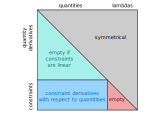
\includegraphics[scale=0.6]{img/implementation/sparse_structure}
    \caption{General Structure of the Systems Jacobian Matrix}
    \label{fig:implementation/sparse_structure}
\end{figure}

\subsubsection{Solution Estimation}\label{subsubsec:solution-estimation}

The estimation of the step solution is a crucial point to ensure fast and reliable convergence of the Newton procedure.

The solution on free surfaces is easily obtained with high precision by first estimating the vacancy concentrations using \autoref{eq:vacancy-concentration}, but expressing the chemical potential by the Gibbs energy gradient of \autoref{eq:gibbs-partial-surface-normal} as in \autoref{eq:chemical-potential-by-gibbs-gradient}.

\begin{equation}
    \Estimated{\Diff\ChemicalPotential} = \frac{\partial\GibbsEnergy}{\partial\Step_{\Normal}} \cdot \frac{2\MolarVolume}{\SurfaceDistance_{\Upper} + \SurfaceDistance_{\Lower}}
    \label{eq:chemical-potential-by-gibbs-gradient}
\end{equation}

Then the fluxes are obtained using Fick's first law (\autoref{eq:fick-first}).
By balancing the fluxes and dividing by the volume gradient, the normal displacement of a node is obtained:

\begin{equation}
    \Estimated{\Step\Shift_{\Normal}} = \left( \Flux_{\Upper} - \Flux_{\Lower} \right) \left( \frac{\partial\Volume}{\partial\Shift_{\Normal}} \right)^{-1}
    \label{eq:estimate-normal-displacement}
\end{equation}

When simulating the evolution of a single particle free in space, this estimate solves the step directly.
A single Newton step is than only needed to obtain the Lagrange multipliers.
When, however, a sinter neck is present, the situation becomes much more complicated, as the neck points feature two modes of displacement with distinct volume and energy gradients and the requirement of maintaining contact.
The issue is solved using a fixed-poit iteration procedure, whose starting point is the simple estimation described above.
The target variable is the flux between the neck node and the central grain boundary node, denoted here as $\Estimated\Flux$.

In the first approximation, the normal displacement of the neck nodes must be equal to that of the grain boundary node to fulfill contact consitions.
Then, the tangetial displacement of the neck node calculates as in \autoref{eq:estimate-neck-tangetial-displacement} using the flux balance there, with $\Flux_{\Surface}$ as the estimated flux to the adjacent surface node calculated as above and $i$ as the iteration index.

\begin{equation}
    \Estimated{\Step\Shift_{\Tangential i}} =
    \left( \Estimated{\Flux_i} - \Flux_{\Surface} - \frac{\partial\Volume}{\partial\Shift_{\Normal}} \Estimated{\Step\Shift_{\Normal i}} \right)
    \left( \frac{\partial\Volume}{\partial\Shift_{\Tangential}} \right)^{-1}
    \label{eq:estimate-neck-tangetial-displacement}
\end{equation}

With this the total dissipation on the neck node is given by:

\begin{equation}
    \Estimated{\Dissipation_i}
    = \frac{\partial\GibbsEnergy}{\partial\Shift_{\Normal}} \Estimated{\Step\Shift_{\Normal i}}
    + \frac{\partial\GibbsEnergy}{\partial\Shift_{\Tangential}} \Estimated{\Step\Shift_{\Tangential i}}
    \label{eq:estimated-neck-dissipation}
\end{equation}

Using the form of the dissipation function in \autoref{eq:dissipation-function-node} the new flux is obtained as in \autoref{eq:estimated-neck-new-flux}.
The signum term is required to support negative dissipations, which occur when the system reaches a stationary state of the surface near the neck in later stages which is characterized by small fluctuations.

\begin{equation}
    \Estimated{\Flux_{i+1}} =
    \sign \Estimated{\Dissipation_i} \cdot
    \sqrt{
        \frac{\MolarVolume{\VacancyConcentration}^\Standard}{\GasConstant\Temperature}
        \frac{\DiffusionCoefficient_{\Upper}}{\SurfaceDistance_{\Upper}}
        \Abs{\Estimated{\Dissipation_i}}
    }
    \label{eq:estimated-neck-new-flux}
\end{equation}

This flux is then inserted in the iteration again in \autoref{eq:estimate-normal-displacement} for the grain boundary nodes and \autoref{eq:estimate-neck-tangetial-displacement} for the neck node till the fixed point is reached.

\section{Calculation and Extraction of Key Features}\label{sec:extraction}
\begin{itemize}
    \item Volume Cell, Shrinkage
    \item Neck Measures
\end{itemize}


    \chapter{Model Validation}\label{ch:model-validation}

\section{Investigations on Simple Test Cases}\label{sec:simple-cases}
\section{Experimental Validation Counter Bulk Sintering Trials}\label{sec:sintering-trials}

    \input{tex/summary_and_outlook}

    %\input{symbol_index}

    \listoffigures
    \listoftables
    \printbibliography

    \appendix
\addpart{Appendix}

\chapter{Equation System}\label{ch:equation-system}


\section{Components of the Lagrangian Gradient}\label{sec:components-of-the-lagrangian-gradient}

The following table displays all components of the Lagrangian gradient to be solved for the application of the \gls{TEP}.
Node symbols $n$ or contact symbols $c$ in parentheses behind another symbol mean, that this symbol is local to the node or contact, thus there exist one distinct value for each node or contact.
$n_\Upper$ denotes the upper neighbor of the currently regarded node, as well as $n_\Lower$ the lower.
The equations are all formulated in terms of fluxes from one node to the upper neighbor $\Flux_{\Upper}$, since $\Flux_\Lower(n) = -\Flux_\Upper(n_\Lower)$ must be always fulfilled.
This saves one unknown per node.

\begin{longtblr}[
    label=none,
    entry=none,
    note{*}={Only if the node is in parent position.}
]{
    colspec={lX[c]},
    measure=vbox
}
    \toprule
    \SetCell[c=2]{l} for each non-contact node $n$ \\
    \midrule
    $\LagrangeFunction_{\Step\Shift_\Normal(n)}$ &
    \begin{equation*}
        0
        = \frac{\partial\GibbsEnergy}{\partial\Shift_\Normal(n)} \left( 1 + \LagrangeParameter_1 \right)
        + \frac{\partial\Volume(n)}{\partial\Shift_\Normal(n)} \LagrangeParameter_{\Volume}(n)
    \end{equation*} \\

    $\LagrangeFunction_{\Flux_\Upper(n)}$ &
    \begin{equation*}
        0
        = \frac{2 \GasConstant \Temperature}{\MolarVolume \VacancyConcentration^\Standard} \frac{\SurfaceDistance_\Upper(n) \Flux_\Upper(n)}{\DiffusionCoefficient_\Upper(n)} \LagrangeParameter_1
        - \LagrangeParameter_\Volume(n)
        + \LagrangeParameter_\Volume(n_\Upper)
    \end{equation*} \\

    $\LagrangeFunction_{\LagrangeParameter_\Volume(n)}$ &
    \begin{equation*}
        0
        = \frac{\partial\Volume(n)}{\partial\Shift_\Normal} \Step\Shift_{\Normal}(n)
        - \Flux_{\Upper}(n)
        + \Flux_{\Upper}(n_\Lower)
    \end{equation*} \\

    \midrule
    \SetCell[c=2]{l} for each contact node $n$ as part of contact $c$ \\
    \midrule
    $\LagrangeFunction_{\Step\Shift_\Normal(n)}$ &
    \begin{equation*}
        0
        = \frac{\partial\GibbsEnergy}{\partial\Shift_\Normal(n)} \left( 1 + \LagrangeParameter_1 \right)
        + \frac{\partial\Volume(n)}{\partial\Shift_\Normal(n)} \LagrangeParameter_{\Volume}(n)
        - \frac{\partial \Radius_\Contact(c)}{\partial\Shift_\Normal(n)} \LagrangeParameter_{\Radius_\Contact}(n)
        - \frac{\partial \Angle_\Contact(c)}{\partial\Shift_\Normal(n)} \LagrangeParameter_{\Angle_\Contact}(n)
    \end{equation*} \\

    $\LagrangeFunction_{\Step\Shift_\Tangential(n)}$ &
    \begin{equation*}
        0
        = \frac{\partial\GibbsEnergy}{\partial\Shift_\Tangential(n)} \left( 1 + \LagrangeParameter_1 \right)
        + \frac{\partial\Volume(n)}{\partial\Shift_\Tangential(n)} \LagrangeParameter_{\Volume}(n)
        - \frac{\partial \Radius_\Contact(c)}{\partial\Shift_\Tangential(n)} \LagrangeParameter_{\Radius_\Contact}(n)
        - \frac{\partial \Angle_\Contact(c)}{\partial\Shift_\Tangential(n)} \LagrangeParameter_{\Angle_\Contact}(n)
    \end{equation*} \\

    $\LagrangeFunction_{\Flux_\Upper(n)}$ & same as above \\

    $\LagrangeFunction_{\LagrangeParameter_\Volume(n)}$ &
    \begin{equation*}
        0
        = \frac{\partial\Volume(n)}{\partial\Shift_\Normal} \Step\Shift_{\Normal}(n)
        + \frac{\partial\Volume(n)}{\partial\Shift_\Tangential} \Step\Shift_{\Tangential}(n)
        - \Flux_{\Upper}(n)
        + \Flux_{\Upper}(n_\Lower)
    \end{equation*} \\

    $\LagrangeFunction_{\LagrangeParameter_{\Radius_\Contact}(n)}$\TblrNote{*} &
    \begin{multline*}
        0
        = \Step\Radius_{\Contact}(c)
        - \frac{\partial \Radius_\Contact(c)}{\partial\Shift_\Normal(n)} \left( \Step\Shift_{\Normal}^{|\Parent}(n) + \Step\Shift_{\Normal}^{|\Child}(n) \right)
        - \frac{\partial \Radius_\Contact(c)}{\partial\Shift_\Tangential(n)} \left( \Step\Shift_{\Tangential}^{|\Parent}(n) + \Step\Shift_{\Tangential}^{|\Child}(n) \right) \\
        - 2 \frac{\partial \Radius_\Contact(c)}{\partial\Shift_\RotationAngle(n)} \Radius^{|\Child}(n) \sin \frac{\Step\RotationAngle_\Child(c)}{2}
    \end{multline*} \\

    $\LagrangeFunction_{\LagrangeParameter_{\Angle_\Contact}(n)}$\TblrNote{*} &
    \begin{multline*}
        0
        = \Step\Angle_{\Contact}(c)
        - \frac{\partial \Angle_\Contact(c)}{\partial\Shift_\Normal(n)} \left( \Step\Shift_{\Normal}^{|\Parent}(n) + \Step\Shift_{\Normal}^{|\Child}(n) \right)
        - \frac{\partial \Angle_\Contact(c)}{\partial\Shift_\Tangential(n)} \left( \Step\Shift_{\Tangential}^{|\Parent}(n) + \Step\Shift_{\Tangential}^{|\Child}(n) \right) \\
        - 2 \frac{\partial \Angle_\Contact(c)}{\partial\Shift_\RotationAngle(n)} \Radius^{|\Child}(n) \sin \frac{\Step\RotationAngle_\Child(c)}{2}
    \end{multline*} \\

    \midrule
    \SetCell[c=2]{l} for each contact $c$ with the therein involved nodes of the parent $\Nodes^{|\Parent}(c)$ \\
    \midrule
    $\LagrangeFunction_{\Step\Radius_\Contact(c)}$ &
    \begin{equation*}
        0
        = \sum^{\Nodes^{|\Parent}(c)}_n \LagrangeParameter_{\Radius_\Contact}(n)
    \end{equation*} \\

    $\LagrangeFunction_{\Step\Angle_\Contact(c)}$ &
    \begin{equation*}
        0
        = \sum^{\Nodes^{|\Parent}(c)}_n \LagrangeParameter_{\Angle_\Contact}(n)
    \end{equation*} \\

    $\LagrangeFunction_{\Step\RotationAngle_\Child(c)}$ &
    \begin{multline*}
        0
        = \sum^{\Nodes^{|\Parent}(c)}_n \Biggl[
            - \Radius^{|\Child}(n) \sin \left( \Step\RotationAngle_\Child(c) + \Angle^{|\Child}(n) - \Angle_\Contact^{|\Child}(c) \right) \LagrangeParameter_{\Radius_\Contact}(n) \\
            + \frac{\Radius^{|\Child}(n)}{\Radius_\Contact(c)} \cos \left( \Step\RotationAngle_\Child(c) + \Angle^{|\Child}(n) - \Angle_\Contact^{|\Child}(c)  \right) \LagrangeParameter_{\Angle_\Contact}(n)
            \Biggr]
    \end{multline*} \\

    \midrule
    \SetCell[c=2]{l} just once for the set of all nodes $\Nodes$ \\
    \midrule
    $\LagrangeFunction_{\LagrangeParameter_1}$ &
    \begin{equation*}
        0
        = \sum^\Nodes_n \left[
            \frac{\partial\GibbsEnergy}{\partial\Shift_\Normal(n)} \Step\Shift_\Normal(n)
            + \frac{\partial\GibbsEnergy}{\partial\Shift_\Tangential(n)} \Step\Shift_\Tangential(n)
            - \frac{\SurfaceDistance_\Upper(n) \Flux_\Upper(n)^2 + \SurfaceDistance_\Lower(n) \Flux_\Upper(n_\Lower)^2}{2\GasConstant\Temperature\MolarVolume\VacancyConcentration^\Standard}
            \right]
    \end{equation*} \\
    \bottomrule
\end{longtblr}


\section{Components of the Lagrangian Gradient's Jacobian}\label{sec:components-of-the-lagrangian-gradients-jacobian}


\end{document}